%%
%% This is file `main.tex',
%% generated with the docstrip utility.
%%
%% The original source files were:
%%
%% samples.dtx  (with options: `manuscript')
%% 
%% IMPORTANT NOTICE:
%% 
%% For the copyright see the source file.
%% 
%% Any modified versions of this file must be renamed
%% with new filenames distinct from main.tex.
%% 
%% For distribution of the original source see the terms
%% for copying and modification in the file samples.dtx.
%% 
%% This generated file may be distributed as long as the
%% original source files, as listed above, are part of the
%% same distribution. (The sources need not necessarily be
%% in the same archive or directory.)
%%
%% The first command in your LaTeX source must be the \documentclass command.
%%%% Small single column format, used for CIE, CSUR, DTRAP, JACM, JDIQ, JEA, JERIC, JETC, PACMCGIT, TAAS, TACCESS, TACO, TALG, TALLIP (formerly TALIP), TCPS, TDSCI, TEAC, TECS, TELO, THRI, TIIS, TIOT, TISSEC, TIST, TKDD, TMIS, TOCE, TOCHI, TOCL, TOCS, TOCT, TODAES, TODS, TOIS, TOIT, TOMACS, TOMM (formerly TOMCCAP), TOMPECS, TOMS, TOPC, TOPLAS, TOPS, TOS, TOSEM, TOSN, TQC, TRETS, TSAS, TSC, TSLP, TWEB.
% \documentclass[acmsmall]{acmart}

%%%% Large single column format, used for IMWUT, JOCCH, PACMPL, POMACS, TAP, PACMHCI
% \documentclass[acmlarge,screen]{acmart}

%%%% Large double column format, used for TOG
% \documentclass[acmtog, authorversion]{acmart}

%%%% Generic manuscript mode, required for submission
%%%% and peer review
% \documentclass[manuscript,screen,nonacm]{acmart}
\documentclass[acmtog,authorversion,nonacm]{acmart}

%%
%% \BibTeX command to typeset BibTeX logo in the docs
\AtBeginDocument{%
  \providecommand\BibTeX{{%
    \normalfont B\kern-0.5em{\scshape i\kern-0.25em b}\kern-0.8em\TeX}}}

%% Rights management information.  This information is sent to you
%% when you complete the rights form.  These commands have SAMPLE
%% values in them; it is your responsibility as an author to replace
%% the commands and values with those provided to you when you
%% complete the rights form.
\setcopyright{acmcopyright}
\copyrightyear{2018}
\acmYear{2018}
\acmDOI{10.1145/1122445.1122456}

%% These commands are for a PROCEEDINGS abstract or paper.
% \acmConference[Woodstock '18]{Woodstock '18: ACM Symposium on Neural
%   Gaze Detection}{June 03--05, 2018}{Woodstock, NY}
% \acmBooktitle{Woodstock '18: ACM Symposium on Neural Gaze Detection,
%   June 03--05, 2018, Woodstock, NY}
% \acmPrice{15.00}
% \acmISBN{978-1-4503-XXXX-X/18/06}
% Hide ACM Reference Format
\settopmatter{printacmref=false}

\renewcommand\footnotetextcopyrightpermission[1]{} % removes footnote with conference info
\setcopyright{none}


%%
%% Submission ID.
%% Use this when submitting an article to a sponsored event. You'll
%% receive a unique submission ID from the organizers
%% of the event, and this ID should be used as the parameter to this command.
%%\acmSubmissionID{123-A56-BU3}

%%
%% The majority of ACM publications use numbered citations and
%% references.  The command \citestyle{authoryear} switches to the
%% "author year" style.
%%
%% If you are preparing content for an event
%% sponsored by ACM SIGGRAPH, you must use the "author year" style of
%% citations and references.
%% Uncommenting
%% the next command will enable that style.
%%\citestyle{acmauthoryear}

\graphicspath{{src/images/}}

%%
%% end of the preamble, start of the body of the document source.
\begin{document}

%%
%% The "title" command has an optional parameter,
%% allowing the author to define a "short title" to be used in page headers.
\title{Literature Review on Novel Indoor Localization Techniques}

%%
%% The "author" command and its associated commands are used to define
%% the authors and their affiliations.
%% Of note is the shared affiliation of the first two authors, and the
%% "authornote" and "authornotemark" commands
%% used to denote shared contribution to the research.
\author{Rubens Luiz Rech Junior}
\email{rluiz@rhrk.uni-kl.de}
\author{Julio Cesar de Azeredo}
\email{deazered@rhrk.uni-kl.de}
\author{Rodrigo Franzoi Scroferneker}
\email{rods@rhrk.uni-kl.de}
\author{Leonardo Eich}
\email{leoeich@rhrk.uni-kl.de}
\author{Kavyashree Renukachari}
\email{}
\affiliation{%
  \institution{Technische Universität Kaiserslautern}
%   \streetaddress{Erwin-Schrödinger-Straße 52}
  \city{Kaiserslautern}
  \state{Rheinland-Pfalz}
  \postcode{67663}
  \country{Germany}
}

% \author{Lars Th{\o}rv{\"a}ld}
% \affiliation{%
%   \institution{The Th{\o}rv{\"a}ld Group}
%   \streetaddress{1 Th{\o}rv{\"a}ld Circle}
%   \city{Hekla}
%   \country{Iceland}}
% \email{larst@affiliation.org}

% \author{Valerie B\'eranger}
% \affiliation{%
%   \institution{Inria Paris-Rocquencourt}
%   \city{Rocquencourt}
%   \country{France}
% }

% \author{Aparna Patel}
% \affiliation{%
%  \institution{Rajiv Gandhi University}
%  \streetaddress{Rono-Hills}
%  \city{Doimukh}
%  \state{Arunachal Pradesh}
%  \country{India}}

% \author{Huifen Chan}
% \affiliation{%
%   \institution{Tsinghua University}
%   \streetaddress{30 Shuangqing Rd}
%   \city{Haidian Qu}
%   \state{Beijing Shi}
%   \country{China}}

% \author{Charles Palmer}
% \affiliation{%
%   \institution{Palmer Research Laboratories}
%   \streetaddress{8600 Datapoint Drive}
%   \city{San Antonio}
%   \state{Texas}
%   \postcode{78229}}
% \email{cpalmer@prl.com}

% \author{John Smith}
% \affiliation{\institution{The Th{\o}rv{\"a}ld Group}}
% \email{jsmith@affiliation.org}

% \author{Julius P. Kumquat}
% \affiliation{\institution{The Kumquat Consortium}}
% \email{jpkumquat@consortium.net}

%%
%% By default, the full list of authors will be used in the page
%% headers. Often, this list is too long, and will overlap
%% other information printed in the page headers. This command allows
%% the author to define a more concise list
%% of authors' names for this purpose.
\renewcommand{\shortauthors}{Rubens L. R. Junior, Júlio C. de Azeredo, Rodrigo F. Scroferneker, Leonardo Eich and Kavyashree Renukachari}

%%
%% The abstract is a short summary of the work to be presented in the
%% article.

\begin{abstract}
  A clear and well-documented \LaTeX\ document is presented as an
  article formatted for publication by ACM in a conference proceedings
  or journal publication. Based on the ``acmart'' document class, this
  article presents and explains many of the common variations, as well
  as many of the formatting elements an author may use in the
  preparation of the documentation of their work.
\end{abstract}

%%
%% The code below is generated by the tool at http://dl.acm.org/ccs.cfm.
%% Please copy and paste the code instead of the example below.
%%
% \begin{CCSXML}
% <ccs2012>
%  <concept>
%   <concept_id>10010520.10010553.10010562</concept_id>
%   <concept_desc>Computer systems organization~Embedded systems</concept_desc>
%   <concept_significance>500</concept_significance>
%  </concept>
%  <concept>
%   <concept_id>10010520.10010575.10010755</concept_id>
%   <concept_desc>Computer systems organization~Redundancy</concept_desc>
%   <concept_significance>300</concept_significance>
%  </concept>
%  <concept>
%   <concept_id>10010520.10010553.10010554</concept_id>
%   <concept_desc>Computer systems organization~Robotics</concept_desc>
%   <concept_significance>100</concept_significance>
%  </concept>
%  <concept>
%   <concept_id>10003033.10003083.10003095</concept_id>
%   <concept_desc>Networks~Network reliability</concept_desc>
%   <concept_significance>100</concept_significance>
%  </concept>
% </ccs2012>
% \end{CCSXML}

% \ccsdesc[500]{Computer systems organization~Embedded systems}
% \ccsdesc[300]{Computer systems organization~Redundancy}
% \ccsdesc{Computer systems organization~Robotics}
% \ccsdesc[100]{Networks~Network reliability}

%%
%% Keywords. The author(s) should pick words that accurately describe
%% the work being presented. Separate the keywords with commas.
\keywords{indoor localization, ubiquitous computing, embedded systems}


%%
%% This command processes the author and affiliation and title
%% information and builds the first part of the formatted document.
\maketitle

\section{Background}

Indoor localization has been an important topic for years and several techniques have been proposed. In \cite{locSysUbiComp}, the authors describe several localization systems, considering aspects of the technologies in which they are based on, their advantages and limitations. In this section, a brief overview of the early indoor localization systems is given.

\subsection{Active Badge}
Developed at the end of the 90s by the Olivetti Research Laboratory, the system used diffuse infrared technology to locate small badges worn by people. Each badge emitted its own unique identifier periodically or on demand. Fixed sensors distributed in the building collected data from the badges and delivered them to a central computer responsible for aggregating the information and computing badge's position. The main limitations of the system were related to the infrared technology, which suffers with interference from fluorescent light and sunlight. Moreover, multiple beacons were needed in larger rooms, because of the limited range of the technology.

\subsection{Active Bat}
The system uses ultrasound time-of-flight for determining distances and lateration technique to locate Active Bats carried by people or objects. First, a central controller sends a radio signal to the Bats which respond transmitting an ultrasound signal. Then, sensors mounted in the ceiling calculate distances using time-of-flight of the receive ultrasound signal and forward them to the central controller that computes Bat's position using trilateration or multilateration. Synchronization is done through a reset signal sent from the controller to the ceiling sensors at the same time as the request signal is emitted via radio to the Bats. The system provides accuracy in the order of centimeters in 95\% of the measurements, but presents problems of scalability, high costs and sensitivity to sensors placement due to the ceiling infrastructure that is needed.

\subsection{Cricket}

\subsection{RADAR}

\subsection{MotionStart magnetic tracker}

\subsection{Easy Living}

\section{Novel Techniques}

\subsection{WiFi-based systems}
% Paper: A Novel Indoor Localization Algorithm for Efficient Mobility Management in Wireless Networks
% Published on: February 2018
% Description written by: Rubens
    The increasing amount of smart devices connected to the Internet wireless raises the challenge of managing network mobility issues. In this context, to track devices' position, specially in indoor environments, plays an essential role in mobility management. Aiming to address these problems, Xiao et al. \cite{Xiao2018} presented an algorithm that fuses multiple signal features to enhance reliability of the  estimated locations and allow more flexible mobility management.
    Most existing works utilize RSS or CSI, exclusively, as the fingerprint of a particular location and this may impede the system from being able to deal with the instability caused by roaming. The authors have observed that, even though CSI might achieve statistically higher accuracy than RSS, for some individual positions, using RSS can provide more accurate estimates. Based on this observation, they propose to combine the results of multiple indoor localization algorithms that use different type of features: Horus \cite{horus}, FIFS \cite{fifs} and D-CSI \cite{d-csi}. Horus is based on RSS data and uses a maximum likelihood approach to estimate locations; FIFS uses aggregated CSI amplitude values over all sub-carriers to leverage on the spatial diversity and enhance performance of RSS-based methods. However, the simple aggregation of all sub-carriers may limit the capability of distinguishing among different positions; D-CSI, instead, uses the distribution of CSI amplitudes and provides better accuracy, since it considers frequency diversity of the sub-carriers and spatial diversity with multiple antennas.
    To obtain devices' locations, two methods are proposed: Fusion 1 and Fusion 2. The former executes Horus and FIFS algorithms and outputs the weighted fusion of their results as the location estimate. The latter selects the 3 most reliable positions among the set of candidate locations generated by Horus, FIFS and D-CSI and calculates the target location as the weighted centroid of these 3 selected locations. The metric used for this selection is based on the proximity of the candidate positions. The methods are shown to improve accuracy in 7\% in the worst case — comparing Fusion 2 to D-CSI — and 31\% in the best case — comparing Fusion 2 with Horus. The median accuracy provided by Fusion 2, which leads to better results, is 0.8 m.
    
% Paper: CSI Phase Fingerprinting for Indoor Localization With a Deep Learning Approach
% Published on: 2016
% Description written by: Julio
    PhaseFi \cite{Wang2016} is the first work to leverage the use of calibrated channel station information (CSI) phase information for indoor fingerprinting. In this work, the probabilistic approach is combined with a deep network model, outperforming three benchmark schemes in both scenarios.
    First, the raw phase information is extracted from CSI and underwent a linear transformation to remove the phase offset. The result of this process is the calibrated phase information, which is considerably more accurate than raw phases. When in the offline stage, the calibrated phase data is trained using a deep network with three hidden layers. In this context, the network's weights represent fingerprints, fully exploiting the essence of the calibrated phase data. Once the fingerprint database is established, the online stage uses a Bayes method based on the radial basis function (RBF) for location estimation.
    The work contributes with a Bayes method for probabilistic location estimation and with a greedy learning algorithm which reduces the complexity of the training phase. Also, for indoor localization accuracy, the experimental results show that PhaseFi based on calibrated phases outperforms all the other schemes (i.e., FIFS, Horus, and ML) \cite{horus, fifs, brunato2005statistical} that are based on amplitudes.
    
% Paper: ConFi: Convolutional Neural Networks Based Indoor Wi-Fi Localization Using Channel State Information
% Published on: 2017
% Description written by: Julio
    The work present on \cite{Chen2017} uses a localization model as a classification problem, addressing it with a five-layer convolutional neural network (CNN). This is the first work to use this kind of network for this task.
    Basically, after collecting the CSI information for the reference points, the data is transformed into a matrix called CSI feature image. This matrix is derived from the CSI data provided by different antennas and sub-carriers.
    The results suggests the capacity of CNN for capturing information in CSI in the indoor localization task. With appropriate parameters, the network outperforms most existing methods, demonstrating the great potential of CNNs to this research subject area.
    
% Paper: Random forest and WiFi fingerprint‑based indoor location recognition system using smart watch
% Published on: 2019
% Description written by: Julio
    Lee \cite{Lee2019} proposed a WiFi-based indoor location recognition using random forest learning. This novel methodology uses Machine Learning methods, Strength Indication (RSSI), and Basic Service Set Identifier (BSSID) to solve the problem of position recognition. The proposed system was demonstrated to have high accuracy and performance.
    To achieve this, the system collects the RSSI, BSSID, and location information through a WiFi sensor inside the indoor area. Based on the collected location data four radio maps are constructed, which
    are regarding the RSSI, BBSID, and location from a WiFi AP for each indoor space grid. Finally, the location information is used as an input in the random forest model, which returns the localization result.
    Although the work did not consider the problem caused by WiFi noise or signal attenuation, the novel methodology proposed demonstrated an improvement in the execution time and accuracy performance. However, the method can be applied to various fields such as logistics, disasters, and IoT services.
    
% Paper: WiDeep: WiFi-based accurate and robust indoor localization system using deep learning
% Published on: 2019
% Description written by: Julio
    On the other hand, WiDeep \cite{Abbas2019} combines a stacked denoising autoencoders deep learning model and a probabilistic framework, used to filter the noise in the WiFi signal and describe the essential characteristics of the relationship between the WiFi APs signals and the mobile location. Its accuracy outperforms the state-of-the-art techniques and is robust to heterogeneous devices.
    The system runs in two phases: offline training phase and online localization phase. During the first one, multiple deep neural networks are created, one for each reference point. This makes the system easy to train and scalable to large areas. After that, the models are stored to be used in the online phase. This phase consists of scanning all APs and their RSSs at the unknowing point. Then, the data are processed and fed into the deep neural networks. Finally, the probabilistic framework receives the networks' results and estimates the user's most probable localization.
    The results show that WiDeep has a great improvement in the accuracy of localization compared with the techniques of the state of the art by at least 53\% for large environments and 29.8\% for small environments. In addition, its performance is robust for different densities of APs in indoor areas and different devices.
    
    
% Paper: ArrayTrack: A fine-grained indoor location system
% Published on: April 2013
% Description written by: Rubens
    The ever-growing application and improvements of MIMO (multiple-input multiple-output) techniques, which has leading to an increase in the number of antennas in the WiFi access points (APs), can be seen as an opportunity to enhance quality of indoor localization systems. Moreover, the high density of APs, still needed to provide good network coverage, can be exploited in the sense that signal transmissions reach several APs, allowing collaboration between them in order to improve accuracy of location estimates. Considering that, ArrayTrack \cite{arrayTrack} is an indoor localization system that uses MIMO based techniques, APs communication and physical layer data — which enables the extraction of information from the received packets even with very low SNR — to obtain an accuracy of 23 cm.
    Upon receiving packets, each AP computes angle of arrival (AoA) spectrum, which is an estimate of signal's power as function of angle of arrival. The system aggregates data from all the APs at a central server that estimates the client's location. Despite the simplicity of these steps, an obstacle for the system arises from the effect of multipath propagation. Because of this phenomena, the direct-path signal — between the user's device and the AP — can be significantly weaker than the reflected signals. Thus, additional signal processing steps are needed to improve accuracy. To address this problem, the authors propose a \textit{multipath suppression} algorithm to remove AoA spectrum peaks that does not correspond to the direct path from client to the AP. It is based on the analysis of changes in the channel properties, caused by movements in the environment, which is done by grouping AoA spectra from multiple frames. Besides that, the system leverages on the *diversity selection* feature of APs — in which the device quickly switches between antennas to improve performance in the presence of destructive multipath fading — to compute multiple AoA info from a single frame. This provides higher diversity for the obtained AoA data, which allows the system to compute more accurate locations, especially in case of low density of APs.
    The overall observation is that the system significantly improves accuracy. The use of FPGAs enables not exacerbating computing latency, which is around 100 ms, even with the complexity of the required signal processing. It is notable that the system outperforms techniques that rely on maps of multipath signal strength, in terms of accuracy, even using fewer APs. It evinces the importance of techniques for mitigating the multipath propagation effects and another benefit of using MIMO technology.

% Paper: Adapting Convolutional Neural Networks for Indoor Localization with Smart Mobile Devices
% Published on: May 2018
% Description written by: Kavya
    Here, a framework presented in \cite{cnn} is discussed. CNN-LOC is a framework that uses Convolutional Neural Network (CNN) based WiFi fingerprinting to deliver a superior level of indoor localization accuracy to a user with a smartphone. CNN-LOC creates input images by using received signal strength indicator (RSSI) of WiFi signals that are then used to train a CNN model, without requiring any specialized hardware/infrastructure. The framework works on a user’s smartphone, within the computational capabilities of the device, and utilizes the radio interfaces for efficient fingerprinting-based localization. 
    
    	\begin{figure}[H]
    		\captionsetup{justification=centering}
    		\includegraphics[scale=0.1]{"cnn_loc_cnn.png"}
    		\caption{An overview of the CNN-LOC framework \cite[Fig. 2]{cnn}}
    	\end{figure}
    	
    An overview of CNN-LOC indoor localization framework is shown in Fig. 2. The framework is divided into two phases. The first phase involves RSSI data collection, cleaning, and pre-processing. This pre-processed data is used to create a database of images. Each image represents a WiFi RSSI based signature that is unique to a location (i.e., x-y co-ordinate). This database of images is used to train a CNN model. The trained model is deployed on a smartphone. In the second phase, real time AP data is converted into an image and then fed to the trained CNN model to predict the location of the user. The CNN model predicts the closest block that was sampled as the users’ location.
    
    \subsubsection{CNN Architecture}
    	\begin{figure}[H]
    		\captionsetup{justification=centering}
    		\includegraphics[scale=0.1]{"cnn_loc_overview.png"}
    		\caption{CNN architecture \cite[Fig. 1]{cnn}}
    	\end{figure}
    	
    The structure of the CNN in CNN-LOC is inspired from the well-known CNN architectures, LeNet \cite{lenet} and AlexNet \cite{alexNet}. CNN architecture used is shown in Fig. 2. Each layer, referred to as [Conv-ReLu], performs a convolution of a small region of the input image with the filter and feeds the result to the ReLu activation function. For the first layer of [Conv-ReLU], 32 filters are used to create a set of 32 feature maps. Five hidden layers of [Conv-ReLU] are used. In the end, a fully connected layer helps in identifying the individual class scores (in our case each class is a unique location). The class with the highest score is selected as the output. In this layer, all the neurons are connected to the neurons in the previous layer (green-dotted-lines).
    
    \subsubsection{Pre-processing of RSSI data} 
    The process of image database creation begins with the collection of RSSI fingerprints. The RSSI for various APs are captured along with the corresponding x and y coordinates at the training locations. Information only for known WiFi APs are maintained to ensure that the trained model is not polluted by unstable WiFi APs. On the RSSI scale, values typically range between -95 dB (lowest) to -0 dB (highest). RSSI values are normalized on a scale from 0 and 100, where 0 represents the weak or null signal, and 100 represents the strongest signal.
        
    Assume that while fingerprinting an indoor location, a total of $K$ APs are discovered at $N$ unique locations. These combine to form a two-dimensional matrix of size $N$ × $K$. Each row vector represents the normalized RSSI fingerprint at the $N_th$ location, denoted as $l_N$, is given by a row vector $[r_1 , r_2, ..., r_K]$, denoted by $R_N$, and each column vector, $[w_1 , w_2 ,..., w_N ]$ represents the normalized RSSI values of the $K_th$ AP at all $N$ locations, denoted by $W_K$. Pearson Correlation Coefficient (PCC) \cite{pcc} between each column vector $W_K$ and the location vector $[l_1 , l_2 , ..., l_N]$. The result is a vector of correlation values denoted as $C$. PCC is useful in identifying the most significant APs in the database that impact localization accuracy. The coefficient values range across a scale of -1 to +1. If the relationship is -1, it represents a strong negative relationship, whereas +1 represents a strong positive relationship, and 0 implies that the input and output have no relationship. APs whose correlation to the output coordinates is below a certain threshold (|PCC| < 0.3) are removed to reduce the computational workload of the framework.
    
    \subsubsection{RSSI Image Database}
    The normalized RSSI data for a given location are converted into a greyscale image. To form greyscale images, a Hadamard Product (HP) \cite{hp} is calculated for each $R$ and $C$. The dimension of each HP is 1 × $K$. Then, the HP matrix is reshaped into a $p x p$ matrix, which represents a 2D image. The HP is padded with zeros in the case that $K$ is less than $p^2$. This set of N images of size $p x p$ are used to train the CNNs. The product's purpose is to promote the impact of the APs that are highly correlated to fingerprinted locations. Even though there may be attenuation of WiFi signals due to multipath fading effects, the image may fade but will likely still have the pattern information retained.
    
    \subsubsection{Hyperparameters}
    The hyperparameters were defined after an analysis particularly on indoor localization problem domain. The results follow.
        \begin{itemize}
            \item \underline{Number of hidden layers}: A large number of hidden layers lead to longer execution times and conversely, fewer hidden layers may produce inaccurate results. 5 layers of [Conv-ReLU] was found to work best for indoor localization domain.
            \item \underline{Size of filter}: This defines the image area that the filter considers at a time, before moving to the next region of the image. A large filter size might aggregate a large chunk of information in one pass. The optimum filter size in was found to be 2×2.
            \item \underline{Stride size}: The amount of pixels a filter moves by is dictated by the stride size. It was set it to 1 because the size of image was very small and thus not to lose any information.
            \item \underline{Number of filters}: Each filter extracts a distinct set of features from the input to construct different feature maps. Each feature map holds unique information about the input image. There were 32 filters in the first layer and were doubled for each subsequent layer up to 256 filters such that both the fourth and fifth layer had 256 filters.
        \end{itemize}

\subsection{Ultrasound-based systems}
% Intro
    Despite RF-based systems being vastly exploited by the research community, they have some limitations in terms of accuracy caused, among other issues, by the effect of multipath fading phenomena. Also, as the sound propagates slower than electromagnetic waves, it is usually cheaper to measure fine-grained distances using acoustic signals rather than using RF. In this context, several indoor localization systems, like Active Bat, Cricket and many others — for example, 3D-LOCUS and Dolphin — have applied acoustic-based techniques in order to leverage these properties of the sound propagation.
% Paper: A novel acoustic indoor localization system employing CDMA
% Published on: May 2012
% Description written by: Rubens
    The system proposed in \cite{us-cdma} aims to use simple and inexpensive devices to provide indoor positioning with accuracy in the order of centimeters using ultrasound (US). The distance between the speakers (fixed to the ceiling) and the objects to be localized (microphones) are measured using ToA information and the locations are estimated using trilateration technique. The objects can be localized with accuracy of 2 cm and 99\% precision.
    Inspired by Dolphin \cite{dolphin}, the system uses DS-CDMA (Direct Sequence Code Division Multiple Access) method and modulate signals using BPSK (Binary Phase Shift Keying). In this scheme, different codes are assigned to each object to be localized and the transmitted signals are encoded using them, allowing multiple simultaneous transmissions to still be separated at the receivers. Gold sequences are utilized for the encoding in order to spread the frequency spectrum of the signals, which makes them more robust against in-band noise. Moreover, the good auto- and cross-correlation properties of these codes minimize the disturbance between simultaneous transmissions and lead to very accurate distance measurements.
    Differently from Dolphin, trilateration is used instead of multilateration. Even though the system acquire 4 distance measurements, which would imply the use of multilateration, the authors proposed two methods of selecting these distances in order to obtain more reliable results using trilateration. The first method computes the location estimate using the center point of 4 others location estimates, which are obtained by the combinations of the 4 measured distances taken 3 at a time. The second method discards the least reliable ToA measurement (smallest value of correlation peak) and uses the other 3 to compute a single and more robust location estimate.
    
\subsection{Optical-based systems}
% Paper: Novel Indoor Localization System Using Optical Camera Communication
% Published on: July 2018
% Description written by: Rubens
    Besides radio-frequency and ultrasound signals, the light has also been used in indoor localization systems. Among the advantages of using Visible Light Communication (VLC) techniques are the capability of providing accuracy in the order of centimeters, the possibility of implementing systems inexpensively and the immunity to RF interference — which allows the use of these systems in sensitive environments like airplanes and hospitals.
    The use of visible light for locating objects — Visual Light Positioning (VLP) — can be split into groups according to the sub-technique on which they are based: proximity, triangulation, fingerprinting or vision analysis. The first 3 use only LEDs and receivers, but they usually need to apply light multiplexing methods, which increases the system complexity. Vision analysis is a promising approach that uses cameras as the receivers and leverages on the spatial separation in order not to need any multiplexing scheme \cite{vlc-survey}. Moreover, it allows asynchronous operation of the devices and still provides high accuracy positioning. The drawbacks are the higher latency in computing the positions and increased cost due to the use of cameras instead of photodiodes.
    The availability of low-cost LEDs, better camera sensors and increasing processing power of the computing units have enable new possibilities and leveraged the popularity of techniques like Optical Camera Communication (OCC) in the research community. In \cite{occ-burbano}, the authors propose the use of LED beacons and medium cost cameras in a OCC-based system the can track location of several devices simultaneously with accuracy of 1.85 cm and latency of 48 ms.
    The system uses LEDs for transmitting identification signals from the devices  — beacons and the objects to be localized — to a camera that is in the ceiling using On-Off Keying modulation. The beacons emit green light, while the objects, red light, for instance. The camera continuously captures images which are processed by a computer. The image processing steps include: binarization of the green and red channels, dilation for finding the dimensions of the light emitting sources and decoding of the identification signals. Then, the pixels are matched with the real environment distances by applying trigonometric relations and the objects' 3D location is obtained from simple trilateration.
    
    \begin{figure}[H]
    	\captionsetup{justification=centering}
    	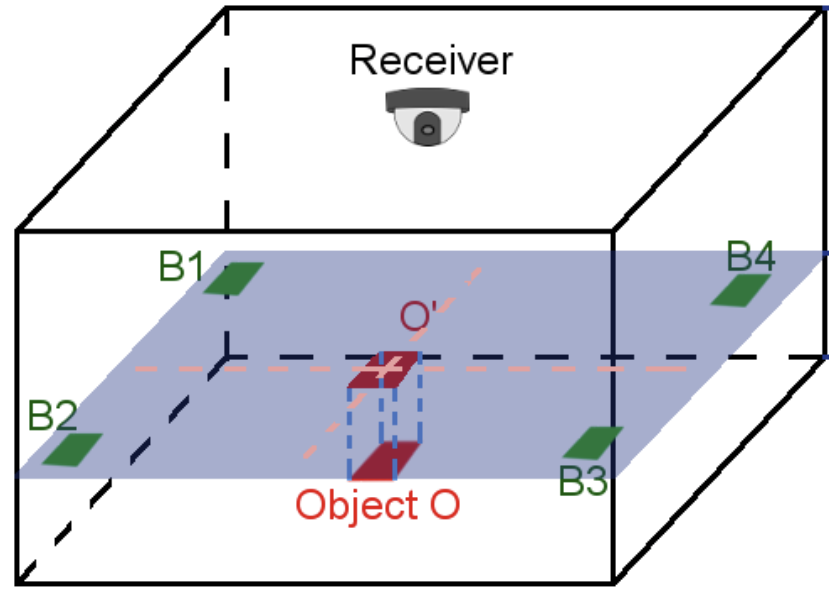
\includegraphics[scale=0.3]{occ-system.png}
    	\caption{Room with several beacons and objects \cite[Fig. 1(a)]{occ-burbano}}
    	\label{fig:occ-burbano}
    \end{figure}
    
    An interesting idea proposed by the authors is to place all the beacons at predefined distance from the camera forming a virtual plane (see Fig.~\ref{fig:occ-burbano}) which incur simplification of the trigonometric relations equations. Moreover, the accuracy of the calculated positions depends on the cameras characteristics and the distance between the beacons and the camera. However, it is notable that, even with simple USB webcam placed at 2 m away from the beacons, the system can provide 3D locations with accuracy of centimeters. 

\subsection{Approaches based on RF Signatures}

% Paper: Indoor Localization for IoT Using Adaptive Feature Selection: A Cascaded Machine Learning Approach
% Published on: November 2019
% Description written by: Kavya
    Here, a novel method presented in \cite{cascade} is discussed. It is based on a cascaded two-stage machine learning approach for highly accurate and robust localization in indoor environments using adaptive selection and combination of RF features. In the proposed method, machine learning is first used to identify the type of the indoor environment based on real data measurements of the RF signal in different indoor scenarios. Then, in the second stage, machine learning is employed to identify the most appropriate selection and combination of RF features that yield the highest localization accuracy.

    \subsubsection{Hybrid RF features}
    Characterizing the type of an indoor environment by a machine learning algorithm becomes a more accurate process when the algorithm makes decisions based on concatenation of RF features of the same environment. In such a way, the accuracy of prediction increases due to the wealth of information available to the algorithm from the multidimensional dataset constructed from the concatenation of the combined RF features of the same environment. Hence, the approach is based on hybrid features. The investigations were carried out using multidimensional information generated from various possible combinations of all or subsets of RSS, CTF, and FCF, which form the hybrid features.
    
    	\begin{figure}[H]
    		\captionsetup{justification=centering}
    		\includegraphics[scale=0.1]{"cascade_umap.png"}
    		\caption{Using hybrid RF features in UMAP algorithm allowed different environments to be classified into distinctive clusters \cite[Fig. 1]{cascade}}
    	\end{figure}
    
    The fifth-dimensional (5-D) hybrid RF feature vector (RSS + CTF + FCF) is mapped into 2-D, with results visualized in Fig. 3. Fig. 3 indicates that the resulting 2-D mapped hybrid RF features vector of the sports hall (open space) is closest to that of the main lobby (low cluttered). Fig. 3 also indicates that the 2-D mapped hybrid RF features vector of the narrow corridor (medium cluttered) is surrounded by that from the main lobby (low cluttered) and lab (highly cluttered). The 2-D embedding of the mapped RF features in Fig. 1 shows that further insights can be gained from the Uniform manifold approximation and projection (UMAP) visualization to confirm the advantage of using the concept of hybrid RF features.
    
    \subsubsection{Data-set and Machine Learning Algorithm}
    A data-set has readings of the RF signal taken in realistic indoor environments of four different types. The frequency domain of CTF, was obtained for four indoor environments: highly cluttered (laboratory), medium cluttered (narrow corridor), low cluttered (lobby), and open space (sports hall).
    
    The machine learning algorithm used is k-NN, which is a non-parametric method used for classification. In this algorithm, the k neighbors of each hybrid RF features vector will determine the type of environment. The k- neighbors are associated with the shortest k Euclidean distances.
    
    \subsubsection{Cascaded Machine Learning Approach}
        \begin{enumerate}
            \item \textit{Machine Learning for Indoor Environment Identification}
            This section is based on work in \cite{cascade_ref1}, \cite{cascade-ref2} where a machine learning approach was used for indoor environment classification based on real measurements of the RF signal. Numerical estimations showed that a machine learning algorithm using k-NN method, utilizing a hybrid combination of CTF and FCF, outperforms other methods, such as decision tree and support vector machine, in identifying the type of the indoor environment with a classification accuracy of 99.3 percent. The accuracy of the adopted technique is represented in terms of the confusion matrix, shown in Fig. 4, for which the diagonal elements represent the percentage of accurate prediction for each type of environment. The off-diagonal elements of the confusion matrix represent the percentage of misclassification.
            
            	\begin{figure}[H]
            		\captionsetup{justification=centering}
            		\includegraphics[scale=0.1]{"cascade_cm.png"}
            		\caption{Confusion matrix using k-NN algorithm (k = 1) based on hybrid RF features CTF + FCF \cite[Fig. 2]{cascade}}
            	\end{figure}
            
            
            \item \textit{Machine Learning for Localization Position Estimation}
            In the second stage and after the type of indoor environment has been identified, a specific selection and combination of RF feature is utilized based on the identified indoor environment. k-NN algorithm has been adopted again in the second stage in order to estimate the sensor position by comparing the testing RF feature to the training database of RF features, with the purpose of finding the best matching entry.
    
            	\begin{figure}[H]
            		\captionsetup{justification=centering}
            		\includegraphics[scale=0.1]{"cascade_hybrid.png"}
            		\caption{Comparison of Localization Distance Error \cite[Table. I]{cascade}}
            	\end{figure}
            	
            Fig. 5 shows the localization distance error, RMSE, using various primary and hybrid RF features. It can be seen that the choice of the best RF signature is dependent on the type of the indoor environment. In the case of the lab, narrow corridor, and lobby, a hybrid RF feature combining CTF + FCF produced the least error RMSE, whereas for the case of the sports hall, a primary RF feature based on FCF has the best performance. These findings clearly indicate the importance of incorporating information on the type of the indoor environment for improving    location estimation.
        \end{enumerate}
    
% Paper: A Novel Real-Time Deep Learning Approach for Indoor Localization Based on RF Environment Identification
% Published on: June 2020
% Description written by: Kavya
    Here, an approach presented in \cite{dl} is discussed. This novel method is based on a two-stage deep learning approach for highly-accurate localization in indoor environments. A CNN is firstly designed to identify the type of the indoor environment using real data measurements characterizing the environment using RF signatures. In the second stage, another CNN is developed to perform localization. Environment identification stage will provide the critical information on environment type that will significantly improve the accuracy of the localization stage. Obtaining such critical knowledge is done through deep learning approach applied on RF signatures, that characterize the physical environment through their definitions which are expressed in terms of the spatial distribution of the power within the environment at hand. In this way, the computation of the RF signatures inherently accounts for the distinctive effects pertaining to each type of indoor physical environment. Two of the most common RF signatures adopted here are CTF and FCF.

    A main advantage of this work is that the design of the two-stage model is based on training of the CNN of each stage on a real dataset obtained from practical RF measurements. The experimental measurements are repeated in four primary indoor environments categorized as: highly cluttered (Laboratory), medium cluttered (Narrow Corridor), low cluttered (Lobby), and open space (Sports Hall). For each type of indoor physical environments, readings of the RF signal must be taken at positions chosen to be not closely distant; but also not far apart in order to ensure that small-scale variations are captured.
    
    \subsubsection{Two-Stage Deep Learning Approach}
    
    	\begin{figure}[H]
    		\captionsetup{justification=centering}
    		\includegraphics[scale=0.1]{"dl_overview.png"}
    		\caption{Proposed two-stage deep learning approach \cite[Fig. 2]{dl}}
    	\end{figure}
    
    The proposed framework is based on a two-stage deep learning approach that uses the RF measurements dataset, as described in the flow chart of Fig. 6. A CNN is developed in the first stage for environment identification, then another CNN is developed in the second stage for indoor localization using the appropriate model associated with the identified environment. 
    
    	\begin{figure}[H]
    		\captionsetup{justification=centering}
    		\includegraphics[scale=0.1]{"dl_detailed.png"}
    		\caption{Description of the CNN two-stage approach \cite[Fig. 3]{dl}}
    	\end{figure}
    
    Fig. 7 shows a more detailed framework for the proposed environment identification and indoor localization using the RF measurements dataset. The dataset is firstly fed into a CNN which consists of two convolution-pooling layers to extract representative features for environment identification in the first stage and indoor localization in the second stage. The extracted features are flattened and fed into a fully-connected layer to get more abstract representations. Then, a softmax classification layer is used for RF environment identification, and a linear regression layer is employed for indoor localization. The four outputs of the softmax layer give the probabilities of identifying the four primary environment types, whereas the two outputs of the linear regression layer produce the 2D position of indoor localization.

\bibliographystyle{ACM-Reference-Format}
\bibliography{references}

\end{document}
\endinput
%%
%% End of file `main.tex'.
